% !TEX TS-program = xelatex
% !TEX encoding = UTF-8 Unicode

% This is a simple template for a LaTeX document using the "article" class.
% See "book", "report", "letter" for other types of document.

\documentclass[11pt]{article} % use larger type; default would be 10pt

\usepackage[utf8]{inputenc} % set input encoding (not needed with XeLaTeX)

%%% PAGE DIMENSIONS
\usepackage{geometry} % to change the page dimensions
\geometry{a4paper} % or letterpaper (US) or a5paper or....

\usepackage{graphicx} % support the \includegraphics command and options

% \usepackage[parfill]{parskip} % Activate to begin paragraphs with an empty line rather than an indent

%%% PACKAGES
\usepackage{paralist} % very flexible & customisable lists (eg. enumerate/compactitem, etc.)
\usepackage{verbatim} % adds environment for commenting out blocks of text & for better verbatim
\usepackage{subfig} % make it possible to include more than one captioned figure/table in a single float
\usepackage{amsmath} % for align* and some math symbols
\usepackage{amssymb} % for mathbb mostly
\usepackage{listings} % for code blocks plus highlighting and stuff 
\usepackage[dvipsnames]{xcolor} % for the colors


%%% SECTION TITLE APPEARANCE
\usepackage{sectsty}
\allsectionsfont{\sffamily\mdseries\upshape} % (See the fntguide.pdf for font help)
% (This matches ConTeXt defaults)

% Dashes instead of dots for compactitem
\renewcommand\labelitemi{-}

%%% CODE STYLE
\lstdefinestyle{codestyle}{
	commentstyle=\color{Gray},
	keywordstyle=\color{RoyalBlue},
	numberstyle=\tiny\color{BrickRed},
	stringstyle=\color{ForestGreen},
	basicstyle=\ttfamily\footnotesize\bfseries,
	breakatwhitespace=false,
	breaklines=true,
	keepspaces=true,
	showspaces=false,
	showstringspaces=false,
	showtabs=false,
	tabsize=4
}
\lstset{style=codestyle}

%%% END Article customizations

\title{CS 162: Assignment 4 Design Document}
\author{Crystal Lee}
\date{} % Activate to display a given date or no date (if empty),
         % otherwise the current date is printed 

\begin{document}
\maketitle

\section{The Problem}
% explain what you think the problem is asking you to do 
% uncertainties and assumptions 
This time we're making a game called ``Escape from CS 162'' which is a maze game. The player's objective is to make it to the immobile Instructor with enough Programming Skills (3) to pass. If they encounter the Instructor without enough skills, they fail the class and thus lose the game. 

The player starts at a random place in the maze, and has to deal with TAs that roam the maze. If the student finds a TA (they are in the same or adjacent squares), then the player would be caught, lose all of their Programming Skills, and ultimately lose the game. The only way to deal with TAs are either to avoid them or to appease them by demonstrating a Programming Skill. Appeasement lasts for 10 turns.

Programming Skills are pickups that are randomly dispersed throughout the maze, but are guaranteed not to spawn where the Instructor is. They also don't stack (only one skill per square). 

The maze is of a size given by the user when they boot up the game. The minimum is a 5x5 but there is no specified maximum. When the maze is a 5x5, there should be four walls total. It is unspecified if there should \textit{always} be four walls, even for bigger board sizes. 

There are no file inputs or outputs this time, just inputs and outputs to terminal. The program gets inputs in the form of moves (characters) from the user and outputs the current board.

\subsection{Extra Credit}
There are two chances for extra credit, which require extra implementation. The first is implementing an AI that plays for you. Though it doesn't seem to need to be a true AI, it still has to have a decent algorithm that attempts to win the game. It should play as the player does, only knowing about the current board (current player, skill, and TA positions). It says nothing about how good the AI's moves are, but perhaps it's better that way...

The other chance is to implement WASD controls such that we don't have to follow every command with an \verb|Enter| key after it. It would make it play much more like a game and less like a program we wrote for class. Essentially, bonus points for smooth gameplay.

\section{Proposed Solution}
% it's the algorithm you use in your solution 
% either a flow chart or pseudocode (don't need both)
% can also include decomposition of the problem and stuff like that (everything in finding the solution as well...)
On a super high level, my implementation has a couple screens: the start screen (with board size), settings screen, and game screen. Each screen is its own object and controls both input from the user and output to the screen. Setup is done by the main function, though, to ensure that the screen isn't initialized multiple times. Below are some notes I made while thinking about the design. It's mostly UI.

\noindent
\begin{figure}[h]
	\centering
	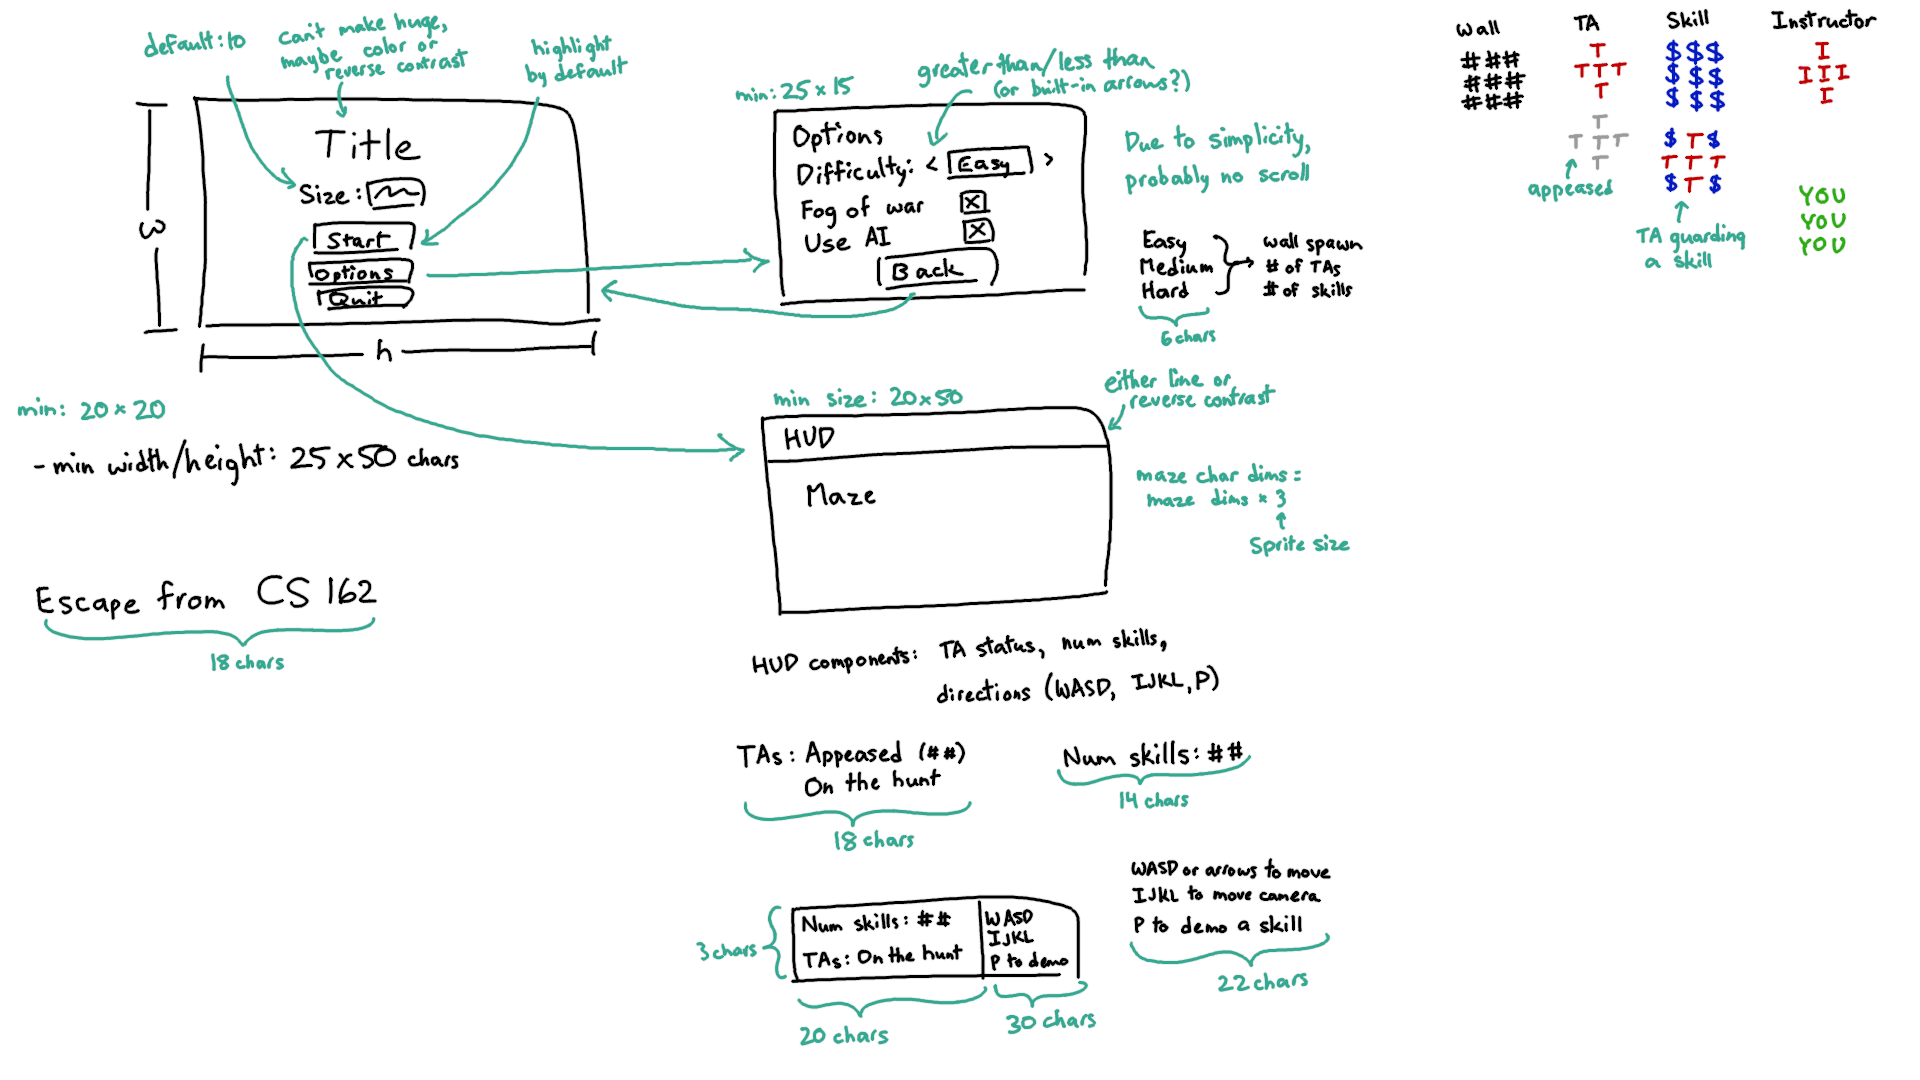
\includegraphics[scale=1]{storyboard.png}
	\caption{Notes for possible UI design.}
\end{figure}

Another note about implementation: there are no animations to handle. That means that everything is driven by user input and the next ``frame'' only changes when the user does something. This means the program doesn't need to deal with handlers for timers or user inputs to change animations or having to worry about frame rate anything like that. The only thing that requires handlers is for screen resizing (from the ncurses library).

\subsection{Main Function}
Arguably the most important function of the entire program: the main function, since it (directly or indirectly) calls everything else from within it. The header is standard, so just the pseudocode is below. The games runs on ``screens'' which are UI elements that point to each other. 

\begin{lstlisting}
initialize window for terminal
make a new GameScreen pointer called currScreen and initialize it to a new StartScreen

while currScreen isn't a nullptr (if it is, the user wanted to exit)
	run currScreen's input loop and store the resulting screen in nextScreen
	delete currScreen
	set currScreen to nextScreen
delete the window
\end{lstlisting}

\subsection{Required Classes}
The classes listed below are all required classes, often with some function or implementation requirements as well. 
\begin{compactitem}
	\item \verb|MazeLocation| (abstract class), which contains \verb|public bool is_occupiable()| and \verb|public char get_display_character()|
	\item \verb|Wall| (extends \verb|MazeLocation|), which always uses \# as a display character
	\item \verb|OpenSpace| (extends \verb|MazeLocation|), which needs standard getters and setters for whether the space contains a student, TA, instructor, or skill
	\item \verb|Maze|, which contains \verb|public Maze(int, int)|, \verb|public ~Maze()|, and \verb|public| \\ \verb|MazeLocation* get_location(int, int)| and must contain vectors instead of normal dynamic arrays (why? For the specs.)
	\item \verb|MazePerson| (abstract class), which contains \verb|public char get_move()|, \verb|public void| \verb|set_location(int, int)|, \verb|public int get_row()|, and \verb|public int get_col()|
	\item \verb|IntrepidStudent| (extends \verb|MazePerson|)
	\item \verb|TA| (extends \verb|MazePerson|)
	\item \verb|Instructor| (extends \verb|MazePerson|)
	\item \verb|Game|, which must contain a maze and the inhabitants of the maze (list of MazePerson objects)
\end{compactitem}

\subsection{GameScreen}
We like top-down design, right? So I'm gonna start with the \verb|GameScreen| class. This is a purely abstract class (some might even call it an \textit{interface}) that defines some methods involving displaying things on screen. Each of them handles screen resizing and printing stuff to screen. The functions inside are listed below with a general description (none have pseudocode because they're all virtual).
\begin{lstlisting}[language=C++]
// should be called when the window resizes so the screen can be updated accordingly
public virtual void* resizeHandler(int sig);

// input/output loop for this screen, run in main
public virtual GameScreen* loop();
\end{lstlisting}

\subsection{Game}
This is the main panel of the entire program, and extends GameScreen. It contains all of the maze related things (a Maze, vector of MazePerson objects) and has some extra fields regarding the state of the game. 

Besides the normal HUD and maze layout, the screen managed by Game can have some alerts (winning or losing screens). These are managed by an internal state which shows whether an alert exists, which influences input (what keys are valid, what do they do) and output (draw maze or alerts). 

The maze can be large. Larger than the terminal output, so some scrolling must be allowed to make sure the user can see all of it easily. This means that there needs to be some controls for it and functionality attached to it. Using IJKL, the user can do the thing. 

Below is the pseudocode for the \verb|loop()| function (defined in GameScreen), probably the most important of the functions in each GameScreen. We assume that the IntrepidStudent is first in the list of MazePerson objects, so that it appears that everything blocks until the user does something. This function requires the \verb|std::istream.peek()| to work properly, which gets the next input char from cin without taking it out of the input buffer. 

\begin{lstlisting}
loop forever
	peek at user input and store the result in a new var (input)
	if we're in the main part of the game
		if the input isn't a move char
			consume the input
			do the camera or move things
			continue to the next loop
		run through every maze person and ask for its move
	otherwise we're in an alert
		consume the input and do what it needs (move the cursor, return, etc)
\end{lstlisting}

\subsection{StartScreen}
This is one of the two secondary panels, this one controlling the start screen. One of these is created on boot, and connects to the other two screens. Just like Game, this screen also has to keep its current state (cursor location, current maze size).

The \verb|loop()| function pseudocode is below.

\begin{lstlisting}
loop forever
	get user input and store the result in a new var (input)
	switch statement with possible user inputs (WASD, digits, space, enter) 
		corresponding functions based on current state (select up/down, return another screen)
\end{lstlisting}

\subsection{OptionsScreen}
This is one of the two secondary panels, this one controlling the options screen. Just like Game, this screen also has to keep its current state (cursor location, current options). On exiting loop, this should always get back to the start screen. It should also write all options to file (for reading from the Game class). 

The \verb|loop()| function pseudocode is below.

\begin{lstlisting}
loop forever
	get user input and store the result in a new var (input)
	switch statement with possible user inputs (WASD, space, enter) 
		corresponding functions based on current state (select up/down, return another screen)
\end{lstlisting}

\subsection{File Format}
To make this easier, the options screen outputs all settings to file. Each option is separated by spaces, and goes in this format: \verb|difficulty fogOfWar aiUse|. Difficulty is represented by an integer (1 for easy, 2 for medium, 3 for hard) and the remaining two are represented by a 0 for false and 1 for true.

If the file is invalid or doesn't exist, the game should default to medium difficulty, no fog of war, and no AI use. 

\section{Test Coverage}
% how do you check that the solution works 
% table format for test cases perhaps?
% can involve a calculator as well 

The easiest way to test this is panel by panel, but all of them should error when the screen is too small. 

\subsection{Start Screen}
Since there's a UI involved, instead of doing this in table format, here's a list of functionalities instead:

\begin{compactitem}
	\item right at boot, the cursor should start at the start button
	\item if all the user does is start the game, should default to a 10x10 maze
	\item clicking W or S should move the selection up or down, respectively, and wrap around 
	\item clicking A, D, or any digit shouldn't do anything when on the start, options, or back button
	\item clicking A or D while on the maze size should decrement or increment the maze size, respectively
	\item clicking space or enter on the maze size shouldn't do anything
	\item clicking space or enter on the start button should boot up a new game of the specified maze size 
	\item clicking space or enter on the options button should show the options screen 
	\item clicking space or enter on the quit button should terminate the program
\end{compactitem} 

\subsection{Options Screen}
Once again, a list: 

\begin{compactitem}
	\item when first opened, the cursor should start at the back button
	\item should have all settings from before (or default settings if nothing has been changed)
	\item clicking W or S should move the selection up or down, respectively, and wrap around 
	\item clicking A or D shouldn't do anything when on the back button or checkbox options 
	\item clicking A or D should make difficulty easier or harder, respectively, when on the difficulty selector
	\item clicking space or enter on the difficulty selector shouldn't do anything
	\item clicking space or enter on a checkbox option should select or deselect the option
	\item clicking space or enter on the back button should return to the start screen 
\end{compactitem} 

\subsection{Maze Screen}
Final one. This one is the most difficult to test for, but here's a huge list for the main part anyway:

\begin{compactitem}
	\item when first opened, the camera should start centered on the player (or AI)
	\item should have the maze size specified on the start screen 
	\item should use all settings from before (or default settings if nothing has been changed)
	\item fog of war makes it so that the player can't see any entities (MazePerson) except within a 5x5 square centered on them
	\item clicking WASD should move the player unless there is a wall or edge of maze (in which case, it skips their turn because they were stupid)
	\item clicking P should activate a programming skill
	\begin{compactitem}
		\item should appease all TAs and make their sprites grayed out 
		\item should see the TA status in the HUD say ``Appeased'' and the number of turns they're appeased for
	\end{compactitem}
	\item if appeased, the TA appeasement turns should count down for every move the user makes (like a usual status effect)
	\item clicking escape should bring up a quit menu (exit to start screen or exit entirely)
	\item if the user hits a TA and the TA isn't appeased, the lose screen should display 
	\item if the user hits a TA and the TA is appeased, the user should be able to continue playing
	\item if the user hits the instructor and they don't have enough Skills, the lose screen should display
	\item if the user hits the instructor and they have enough Skills, the win screen should display
	\item clicking space or enter should skip the user's turn (they didn't want to move)
\end{compactitem} 

As for any alert dialogs that could pop up, they should disable all inputs to the actual maze portion. It should be WASD for moving the cursor around the options and space or enter for selecting. 

\bigbreak\bigbreak\bigbreak\noindent
Was that enough...? I wanted to start on this assignment ASAP... so I forwent a lot of the usual header plus pseudocode things so I could actually start coding.

\end{document}
